\let\negmedspace\undefined
\let\negthickspace\undefined
\documentclass[journal]{IEEEtran}
\usepackage[a5paper, margin=10mm, onecolumn]{geometry}
\usepackage{lmodern} % Ensure lmodern is loaded for pdflatex
\usepackage{tfrupee} % Include tfrupee package

\setlength{\headheight}{1cm} % Set the height of the header box
\setlength{\headsep}{0mm}     % Set the distance between the header box and the top of the text
\usepackage{multicol}
\usepackage{gvv-book}
\usepackage{gvv}
\usepackage{cite}
\usepackage{amsmath,amssymb,amsfonts,amsthm}
\usepackage{algorithmic}
\usepackage{graphicx}
\usepackage{textcomp}
\usepackage{xcolor}
\usepackage{txfonts}
\usepackage{listings}
\usepackage{enumitem}
\usepackage{mathtools}
\usepackage{gensymb}
\usepackage{comment}
\usepackage[breaklinks=true]{hyperref}
\usepackage{tkz-euclide} 
\usepackage{listings}
% \usepackage{gvv}                                        
\def\inputGnumericTable{}                                 
\usepackage[latin1]{inputenc}                                
\usepackage{color}                                            
\usepackage{array}                                            
\usepackage{longtable}                                       
\usepackage{calc}                                             
\usepackage{multirow}                                         
\usepackage{hhline}                                           
\usepackage{ifthen}                                           
\usepackage{lscape}
\usepackage{tikz}
\begin{document}

\bibliographystyle{IEEEtran}
\vspace{3cm}

\title{2021-EE}
\author{EE24BTECH11060 - sruthi bijili}
% \maketitle
% \newpage
% \bigskip
{\let\newpage\relax\maketitle}

\renewcommand{\thefigure}{\theenumi}
\renewcommand{\thetable}{\theenumi}
\setlength{\intextsep}{10pt} % Space between text and floats


\numberwithin{equation}{enumi}
\numberwithin{figure}{enumi}
\renewcommand{\thetable}{\theenumi}
\begin{enumerate}
    \item In the given circuit,for the maximum power to br delivered to $R_{L}$, its value should be \dots $\ohm$\\
\begin{circuitikz}
    % Voltage source with frequency label beside it
    \draw (0,0) to[sinusoidal voltage source, l_=$V$] (0,3);
    % Adjust label position to the right of the voltage source
    \node[right] at (0.5,2) {$\omega = 1\,\text{k rad/s}$};  % Placed to the right of the voltage source

    % Inductor at the top
    \draw (0,3) to[L=$4\,\text{mH}$] (4,3);  % Increased width by moving to x=4

    % Parallel 2-ohm resistor and load resistor
    \draw (4,3) to[R=$2\,\Omega$] (4,0);  % Adjusted x-coordinate for the resistor
    \draw (4,3) -- (6,3) to[R=$R_L$] (6,0) -- (4,0);  % Resistor moved further right

    % Capacitor below
    \draw (0,0) to[C=$0.5\,\text{mF}$] (4,0);  % Increased width here too
\end{circuitikz}
    \item One coulomb of point charge moving with a uniform velocity $10$ $\hat{x}$ $\frac{m}{s^2}$ enters the region $x$ $\geq$ $0$ having a magnetic flux density $\Bar{B}$=$10y\hat{x}+10x\hat{y}+10\hat{z}$ T. The magnitude of force on the charge at $x$=$0^+$ is \dots N.\\
    $\hat{x}$,$\hat{y}$ and $\hat{z}$ are the unit vectors along x-axis,y-axis and z-axis respectively
    \item Consider a large parallel plate capacitor. The gap $d$ between the two plates is filled entirely with a dielectric slab of relative permittivity $5$.The plates are initially charged to a potential difference of $V$ volts and the then disconnected from the source. If the dielectric slab is pulled out completely,then the ratio of the new electric field $E_{2}$ in the gap to the original electric field $E_{1}$ is\dots
    \item Consider a continuous-time signal $X\brak{t}$ defined by $X\brak{t}=0$ for $\abs{t}$ \textgreater $0$,and $X\brak{t}$=$1-\abs{t}$ for $\abs{t}\leq 1$.Let  the fourier transform of $X\brak{t}$ be defined as $X\brak{\omega}$=$\int_{-\infty}^{\infty} x\brak{t}e_{-jwt} dt$.The maximum magnitude of $X\brak{\omega}$ is \dots.
    \item A belt-driven $DC$ shunt generator running at $300$RPM delivers $100$kW to a $200 V$.Ignoring armature reaction,the speed of the motor is \dots RPM.
   \item An $8$-pole $50$Hz,three-phase,slip-ring induction motor has an effective rotor resistance of $0.08\ohm$ per phase. Its speed at maximum torque is $650$ RPM. The additional resistance per phase that must be inserted in the rotor to achieve maximum torque at start is \dots $\ohm$.Neglect magnetizing current and stator leakage impedance. Consider equivalent circuit parameters referred to stator.
    \item Consider a closed-loop system as shown.$G_{p}\brak{S}$=$\frac{14.4}{s\brak{1+0.1s}}$ is the plant transfer function and $G_{e}\brak{s}=1$ is the compensator. For a unit-step input,the output response has damped oscillations. The damped natural frequency is \dots $\frac{rad}{s}$.\\
   \begin{tikzpicture}[auto, node distance=1.5cm,>=latex']
    % Nodes
    \node [name=input] {};
    \node [right of=input, node distance=0.5cm] (r) {$R(s)$};
    \node [draw, circle, right of=r, node distance=1cm] (sum) {+};
    \node [draw, rectangle, right of=sum, node distance=1.5cm] (Gc) {$G_c(s)$};
    \node [draw, rectangle, right of=Gc, node distance=2.5cm] (Gp) {$G_p(s)$};
    \node [right of=Gp, node distance=2cm] (c) {};
    
    % Labels
    \node [above of=Gc, node distance=0.5cm] {$E(s)$};
    \node [above of=c, node distance=0.5cm] {$C(s)$};
    
    % Lines
    \draw [->] (r) -- (sum);
    \draw [->] (sum) -- (Gc); % Direct line from sum to Gc
    \draw [->] (Gc) -- (Gp);
    \draw [->] (Gp) -- (c) -- ++(0.5,0); % Extend the line after Gp(s)
    \draw [->] (c) |- ++(0,-1.5cm) -| node[pos=0.95] {$-$} (sum);

\end{tikzpicture}

    \item In the given figure, plant $G_{p}\brak{s}$=$\frac{2.2}{\brak{1+0.1s}\brak{1+0.4s}\brak{1+1.2s}}$ and compensator $G_{e}\brak{s}$=$k\brak{\frac{
    1+T_{1}s}{1+T_{2}s}}$.The external disturbance input is $D_{s}$. It is desired that when the disturbance is a unit step,the steady-state error should not exceed $0.1$ unit. The minimum value of $K$ is\dots\\
\begin{tikzpicture}[auto, node distance=2cm, >=latex']

    % Define custom node styles
    \tikzstyle{input} = [coordinate]
    \tikzstyle{sum} = [draw, circle, minimum size=0.6cm]  % Smaller circles for sum blocks
    \tikzstyle{block} = [draw, rectangle, minimum height=1cm, minimum width=2cm]
    \tikzstyle{output} = [coordinate]

    % Nodes
    \node [input, name=input] {};
    \node [sum, right of=input, node distance=1cm] (sum1) {};
    \node [block, draw, right of=sum1] (Gc) {$G_c(s)$};
    \node [sum, right of=Gc, node distance=2cm] (sum2) {};
    \node [block, draw, right of=sum2] (Gp) {$G_p(s)$};
    \node [output, right of=Gp, node distance=2cm] (output) {};
    \node [above of=sum2, node distance=1cm] (disturbance) {$D(s)$};

    % Circles (Nodes)
    \node [coordinate, right of=input, node distance=1cm] (circle1) {}; % Small circle between R(s) and sum1
    \node [coordinate, right of=Gc, node distance=2.2cm] (circle2) {}; % Small circle between Gc and Gp

    % Connections
    \draw [->] (input) -- node {$R(s)$} (circle1) -- (sum1); % Connection with circle1
    \draw [->] (sum1) -- node {$E(s)$} (Gc);
    \draw [->] (Gc) -- (circle2) -- (sum2); % Connection with circle2
    \draw [->] (sum2) -- (Gp);
    \draw [->] (Gp) -- node [name=y] {$C(s)$} (output);
    \draw [->] (y) |- ++(0, -2) -| (sum1) node[pos=0.25, right] {$-$};
    \draw [->] (disturbance) -- (sum2);

\end{tikzpicture}

    \item The waveform shown in the solid line is obtained by clipping a full-wave rectified sinusoidal.The ratio of the RMS value of the full-wave rectified waveform to the RMS value of the clipped waveform is \dots\\
\begin{tikzpicture}
    % Axis
    \draw[->] (-0.5, 0) -- (10, 0) node[right] {$\omega t$};
    \draw[->] (0, -1) -- (0, 2) node[above] {$V_m$};
    
    % Voltage levels
    \draw[dashed] (-0.5, 1.06) -- (10, 1.06) node[right] {$0.707V_m$};  % Keeping the original dashed line at 0.707Vm
    \draw[dashed] (-0.5, 1.5) -- (10, 1.5) node[right] {$V_m$};  % Keeping the original dashed line at Vm

    % Time markers and labels (below the x-axis)
    \foreach \x/\label in {1.57/$\frac{\pi}{4}$, 2.36/$\frac{3\pi}{4}$, 3.14/$\pi$, 6.28/$2\pi$, 9.42/$3\pi$}
        \draw[dashed] (\x, 0) -- (\x, -0.5) node[below] {\label};
    
    % Waveform (sawtooth with sinusoidal tops)
    \draw[thick] (0,0) -- (1.57, 1.5) -- (2.36, 1.5) -- (3.14, 0);
    \draw[thick] (3.14,0) -- (4.71, 1.5) -- (5.5, 1.5) -- (6.28, 0);
    \draw[thick] (6.28,0) -- (7.85, 1.5) -- (8.64, 1.5) -- (9.42, 0);

    % Sinusoidal tops (flipping negative parts above x-axis)
    \draw[dotted, domain=0:3.14, samples=100] plot(\x, {1.5 * sin(\x r)});
    \draw[dotted, domain=3.14:6.28, samples=100] plot(\x, {-1.5 * sin(\x r)});  % Flip negative part
    \draw[dotted, domain=6.28:9.42, samples=100] plot(\x, {1.5 * sin(\x r)});
\end{tikzpicture}

    \item The state space representation of a first-order system is given as \\
    $x$=$-x+u$\\
    $y$=$x$\\
    where,$x$ is the state variable,$u$ is the control input and $y$ is the controlled output. Let $u$=$-kx$ be the control law,where $K$ is the controller gain. To place a closed-loop pole at $-2$,the value of $K$ is\dots
    \item An air-core radio-frequency transformer as shown has a primary winding and a secondary windingand connect an AC source across the transformer and connect other end to the resistor. The mutual inductance $M$ between the windings of the transformer is \dots $\mu$H.\\
 
\begin{circuitikz}

% AC source (without 100 kHz label)
\draw (0,0) node[vsource, invert] (V) {}; 

% Directly connect the AC source to the transformer
\draw (V) -- ++(0,0) node[transformer, yscale=1] (T) {}; 

% Secondary winding of transformer with center tap
\draw (T.B1) ++(0.5,-0.5) node[below] {7.3 V$_{\text{p-p}}$};  % Slightly right and down
\draw (T.B2) ++(0,-1.25) node[below] {5.0 V$_{\text{p-p}}$};  % Moved further down

% Connect the resistor to the bottom end of the left transformer (T.A2)
\draw (T.A2) -- ++(0,-1) to[R=22~$\Omega$] ++(0,-1) node[ground] {};

% Movable indicator "M"
\draw (T) ++(0,1.5) node[] {M};

\end{circuitikz}


    \item A $100Hz$ square wave,switching between $0 V$ and $5 V$,is applied to a CR high-pass filter circuit as shown.The output voltage waveform across the resistor is $6.2 V$ peak-to-peak. If the resistance $R$ is $820 \ohm$,then the value of $C$ is \dots $\mu F$.\\
\begin{circuitikz}
    % Draw the input label and initial node
    \draw 
    (0,0) node[left] {input} 
    -- (0.5,0) % Initial horizontal line to the first node
    node[circle, fill, inner sep=1pt] {} % Node at the left end of C
    to[C=$C$] (2,0) % Capacitor labeled C
    -- (3,0) % Horizontal line to the output
    node[right] {output}; % Output label

    % Draw resistor and node
    \draw 
    (2,0) % Start from the right node of capacitor
    to[R=$R$] (2,-2) % Draw resistor downward
    node[circle, fill, inner sep=1pt] {}; % Node at the bottom of R

    % Draw parallel line starting from the bottom of the resistor
    \draw (2,-2) -- (0.5,-2)  % Extend left to the capacitor node
          (2,-2) -- (3,-2);   % Extend right to the output
\end{circuitikz}


    \item A CMOS schmitt-trigger inverter has a low output level of $0 V$ and a high output level of $5 V$. It has input thresholds of $1.6 V$ and $2.4 V$. The input capacitance and output resistance of the schmitt-trigger are negligible. The frequency of the oscillator shown in \dots $Hz$.\\
 \begin{circuitikz}
    % Draw capacitor to ground
    \draw (0,0) to[C=47\,nF] (0,-2) node[ground]{};
    
    % Draw resistor
    \draw (0,0) to[R=10\,k$\Omega$] (2,0);

    % Draw Schmitt trigger in parallel with the resistor
    \draw (0,0) -- (0,1) -- (2,1) 
    (2,1) -- (2.5,1)
    (2.5,0.5) -- (2.5,1.5) -- (3.5,1) -- (2.5,0.5)
    (3.5,1) -- (4,1);  % Output of the Schmitt trigger

    % Add the hysteresis symbol inside the Schmitt trigger
    \draw (2.8,1.1) -- (3.2,1.1);
    \draw (2.8,0.9) -- (3.2,0.9);

    % Connect the output line from the resistor
    \draw (2,0) -- (4,0);

    % Extend the Schmitt trigger output down to connect to the resistor output
    \draw (4,1) -- (4,0);
    
    % Extend the output line to the right side of the Schmitt trigger
    \draw (4,0) -- (5,0); % Extended line
\end{circuitikz}


\end{enumerate}
\end{document} 
